
\documentclass{sig-alternate}

\usepackage{tikz}
\usetikzlibrary{shapes,arrows}

% Define block styles
\tikzstyle{decision} = [diamond, draw, fill=blue!20, 
    text width=4.5em, text badly centered, node distance=3cm, inner sep=0pt]
\tikzstyle{block} = [rectangle, draw, fill=blue!20, 
    text width=6em, text centered, rounded corners, minimum height=4em]
\tikzstyle{goal_block} = [rectangle, draw, fill=blue!20, 
    text width=0.95\columnwidth, text centered, rounded corners, minimum height=4em]
\tikzstyle{process_block} = [rectangle, draw, fill=blue!20, 
    rounded corners]
\tikzstyle{line} = [draw, -latex']
\tikzstyle{cloud} = [draw, ellipse,fill=red!20, node distance=3cm,
    minimum height=2em]
\hyphenation{In-stru-ct-ion-al}
\begin{document}

\setcopyright{rightsretained}
\conferenceinfo{SIGCSE '16,}{March 2--5, 2016, Memphis, TN, USA.}
\isbn{978-1-4503-3685-7/16/03}
\doi{http://dx.doi.org/10.1145/2839509.2844674}
%Authors, replace the red X's with your assigned DOI string.

\clubpenalty=10000 
\widowpenalty = 10000

\title{Instructional Design is to Teaching as\\Software Engineering is to Programming}
\numberofauthors{1}
\author{
	\alignauthor {Austin Cory Bart and Clifford A. Shaffer}\\
	\affaddr{Virginia Tech}\\
    \email{\{acbart, shaffer\}@vt.edu}\\
}

\maketitle

% A category with the (minimum) three required fields
\category{K.3.2}{Computer and Information Science Education}{Computer Science Education}

\terms{Design, Human Factors}

\keywords{Instructional Design; Teaching; Software Engineering; Dick \& Carey; Formal Methods} % NOT required for Proceedings

\section{Summary}

This special session will explore practical results from 
the educational theory of Instructional Design (ID), with particular focus on the widespread similarities between a process for creating successful courses and a process for creating successful software.
We present a small set of specific practices that should be easy for CS educators to adopt.
In particular, the session will cover the popular Dick \& Carey model, meant for beginners to ID.
This model helps instructors rigorously define \textit{who} they will teach to, \textit{what} they will teach, \textit{how} they will assess, and (only then) \textit{how} they will teach.
The approach is parallel to Software Engineering techniques such as Test-Driven Development, Requirements Engineering, and Iterative Development.

The session will be a blend of presentation, participation, and assessment.
Participants will work in small groups both to foster discussion and to provide learning support.
The content of the presentation will particularly focus on how the model can be applied practically.
It is our hope that attendees, whether new to teaching or experienced, will adopt or be influenced by the model in order to approach their courses with the same rigor they apply to software development.

\section{Objective}

Instructional Design is the iterative, systematic design of effective learning experiences by following a coherent process that gives measurable results.
Its history stretches back into the 1930s~\cite{dick2005systematic}, but there has been surprisingly few published cases of its use in Computer Science Education.
Going the other way, there is a body of research on how Software Engineering techniques can be applied to ID~\cite{douglas-ooid, douglas-seid, tripp-rpid}.
Within CS, what little research that exists focuses on pedagogical tools and tactics~\cite{damian-id, hadjerrouit-id} rather than holistic, cohesive processes.

Figure~\ref{dick-carey-overview} gives an overview of the phases of the Dick \& Carey Model.
Notice that the actual development and testing of instructional materials and strategy is saved for the final phases of the model, rather than the beginning.
Instead, instructors begin by analyzing their ``users'' (the learners) and their instructional goals, then determine concrete objectives and measurements (tests), and finally focus on design and development.
Similar to how Software Engineering does not dictate architecture but rather focuses on process, such as how to do documentation and testing, ID promotes process for things like documentation and organization over constricting your pedagogy.
ID is compatible with other popular educational theories, including Constructivist Learning, Active Learning, and Collaborative Learning.

We will present a number of beneficial strategies with specific implementation recommendations, including:
\begin{description}
\item[Course Alignment ($\approx$ Quality Management)] 
ID leads to explicit definitions for learning objectives, assessments, and course activities, making it clear how components fit together.
\item[Templated Instruction ($\approx$ Design Patterns)] Develop\-ment of instructional strategy and material can be guided by templates.
\item[Assessment Evaluation ($\approx$ Unit Testing)] Instructional faults can be pinpointed, and further isolated and resolved by using techniques such as Item Response Theory to increase the coverage and validity of the assessment instruments.
\item[Course Documentation ($\approx$ Design Documentation)] Good instructional design practice is self documenting.
Collaborators can be given more than the course materials. They can get instructional strategy, assessments, and the rationale behind the instruction.
\end{description}

This session will be organized as a blend of tutorial and hands-on, small-group exercise.
We will introduce a new, practical educational theory to attendees, many of who may be unfamiliar with it.
ID should resonate with instructors that have an engineering background and yearn for similar structure in their design of learning experiences.

\begin{figure*}
\begin{center}
	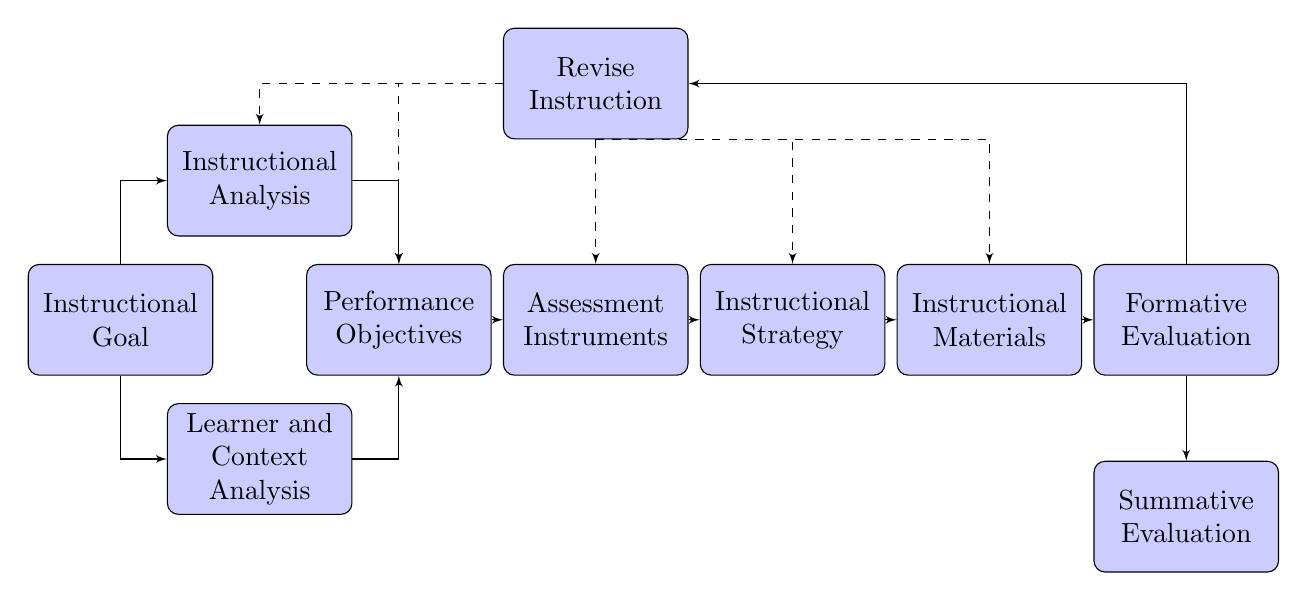
\begin{tikzpicture}[node distance = 2.5cm, auto]
			% Place nodes
			\node [block] (ig) {Instructional Goal};
			\node [block, above right of=ig] (ia) {Instructional Analysis};
			\node [block, below right of=ig] (lc) {Learner and Context Analysis};
			\node [block, below right of=ia] (po) {Performance Objectives};
			\node [block, right of=po] (ai) {Assessment Instruments};
			\node [block, right of=ai] (is) {Instructional Strategy};
			\node [block, right of=is] (im) {Instructional Materials};
			\node [block, right of=im] (fe) {Formative Evaluation};
			\node [block, below of=fe] (se) {Summative Evaluation};
			\node [block, above of=ai, node distance= 3cm] (ri) {Revise Instruction};
			% Draw edges
			\path [line] (ig.north) |- (ia.west);
			\path [line] (ig.south) |- (lc.west);
			\path [line] (lc.east) -| (po.south);
			\path [line] (ia.east) -| (po.north);
			\path [line] (po.east) -- (ai.west);
			\path [line] (ai.east) -- (is.west);
			\path [line] (is.east) -- (im.west);
			\path [line] (im.east) -- (fe.west);
			\path [line] (fe.south) -- (se.north);
			\path [line] (fe.north) |- (ri.east);
			\path [line, dashed] (ri.west) -| (ia.north);
			\path [line, dashed] (ri.west) -| (po.north);
			\path [line, dashed] (ri.south) -| (ai.north);
			\path [line, dashed] (ri.south) -| (is.north);
			\path [line, dashed] (ri.south) -| (im.north);
			%\path [line] (identify) -- (evaluate);
			%\path [line] (evaluate) -- (decide);
			%\path [line] (decide) -| node [near start] {yes} (update);
			%\path [line] (update) |- (identify);
			%\path [line] (decide) -- node {no}(stop);
			%\path [line,dashed] (ia) -- (ig);
			%\path [line,dashed] (lc) -- (ig);
			%\path [line,dashed] (lc) |- (evaluate);
	\end{tikzpicture}
	\caption{The Dick \& Carey Model of Instructional Design}
	\label{dick-carey-overview}
\end{center}
\end{figure*}

\newpage
\section{Outline}

\begin{description}
\item[Introduction:] (15 minutes) Overview of the ID model, its pros and cons, and practical strategies for using it.
\item[Case Study:] (15 minutes) Walk through of the Dick \& Carey model and our experiences using it.
\item[Practice Problems:] (20 minutes) Small group exercise. Attendees will get to apply the model to solidify their knowledge.
\item[Post-Test:] (15 minutes) Attendees will be given a brief, optional ``post-test'' to help them identify if they learned the material of the session.
\item[Discussion:] (10 minutes) Attendees will discuss how the model could be applied to their own classrooms, and their reaction to this special session.
\end{description}

\section{Expectations}

The expected audience is computer science instructors, although anyone interested in educational theory should find the session useful.
No prior experience with ID is expected.
This session will cover an overview of the Dick \& Carey model and demonstrate how it can be used in Computer Science classrooms at any grade level (K-12, undergraduate, etc.), any experience level, and any setting.
We expect that instructors with prior knowledge of ID will also benefit from exposure to this concrete method.

The session will cover how instructors can get more information about the model, to promote long-term transfer of the material.
Feedback will be solicited from attendees using a survey, and there will also be a pre- and post- assessment (both meant as a formative evaluation of the materials and to guide attendees' learning).

\section{Suitability for a Special Session}

The presenters believe that this session is particularly suitable as a Special Session rather than a paper or panel because it requires hands-on experience and sufficient time to do so.
Although a workshop would be a suitable alternative to this format, we suspect that few attendees will be sufficiently knowledgeable of Instructional Design to be willing to invest money in attending it.
But we hope that after initial exposure, instructors will be motivated to learn more.
The Special Session format allows us to provide the SIGCSE community with a low-stakes introduction to a powerful new technique that could revolutionize the way we design our lessons.

\section{Acknowledgment}

This material is based upon work supported by The National Science Foundation Graduate Research Fellowship, Grant No. DGE 0822220


\bibliographystyle{abbrv}
\bibliography{references} 

\end{document}
